\documentclass{beamer}

\usepackage{graphicx}

\begin{document}
%=====================================================%
\begin{frame}
Consider the IP:
\begin{figure}
\centering
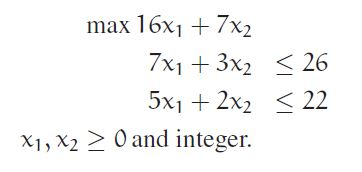
\includegraphics[width=0.7\linewidth]{Exam14-Question}

\end{figure}
\end{frame}

%=========================================== %
\begin{frame}
	\begin{figure}
\centering
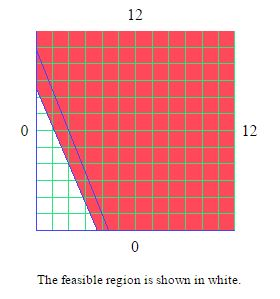
\includegraphics[width=0.7\linewidth]{Exam14-Main}
\end{figure}

\end{frame}
%========================================================================= %

% Vertex        Lines Through Vertex   Value of Objective
% (0,8.666667)  7x+3y = 26; x = 0      60.666667 Maximum
% (3.714286,0)  7x+3y = 26; y = 0      59.428571
% (0,0)         x = 0; y = 0           0

%=========================================================================%
\begin{frame}
\large
\begin{itemize}
\item You will be asked to partly solve the IP, using the Branch and Bound
Method. 
\item You should draw an enumeration tree/diagram to keep
track of your progress — draw the enumeration tree on an otherwise
blank page.
\end{itemize}
\end{frame}
%==========================================================================%
\begin{frame}
\large
\begin{itemize}
\item You will be asked to partly solve the IP, using the Branch and Bound Method.
\item You should draw an enumeration tree/diagram to keep track of your
\item progress — draw the enumeration tree on an otherwise blank page.
\end{itemize}
\end{frame}
%==========================================================================%
\begin{frame}
The corresponding Simplex Tableau (transforming the max problem into a
min problem) is:
\begin{figure}
\centering
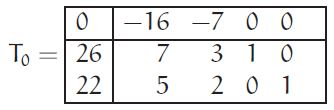
\includegraphics[width=0.7\linewidth]{Exam14-a}
\end{figure}

\end{frame}
%==========================================================================%

\begin{frame}

The columns are for $x_1$,$x_2$, $s_1$ and $s_2$. 
$S_1$ and $s_2$ are called slack variables.

\begin{itemize}
\item $7x1 + 3x2 \leq 26$  
\item $5x1 + 2x2 \leq 22$
\end{itemize}
\end{frame}

%==========================================================================%

\begin{frame}
\begin{itemize}
\item In contrast to the material used in Week 11 , the indicator row is listed at the top of the tableau
\item The $b$ column is listed on the left hand side of the tableau
\end{itemize}
\end{frame}
%==========================================================================%
\begin{frame}
\begin{quote}
N.B. The Simplex Method and the Dual Simplex Method are stated on
the last page of this paper.
You will partly solve the IP, following the steps on the next pages — remember
to draw and fill in an enumeration tree.
\end{quote}
\end{frame}
%==========================================================================%
\begin{frame}
\begin{itemize}
\item[(i)] Apply one iteration of the Simplex Method to the starting tableau
(T0) and show that the Simplex Tableau now takes the form (just
calculate the first 3 columns): 3\%
\end{itemize}

\end{frame}
%============================================== %
\begin{frame}
\begin{figure}
\centering
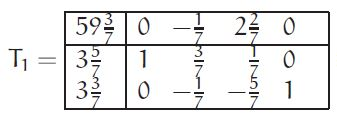
\includegraphics[width=0.7\linewidth]{Exam14-b}\\
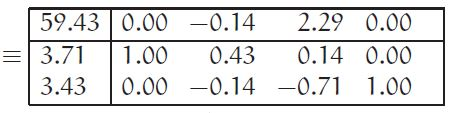
\includegraphics[width=0.7\linewidth]{Exam14-c}
\end{figure}
\end{frame}
%===============================================%
\begin{frame}
\begin{itemize}
\item[(ii)] After a second iteration of the Simplex Method the Simplex Tableau
now takes the form: (N.B. Do not perform the arithmetic!)
\end{itemize}

\begin{figure}
\centering
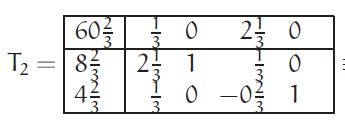
\includegraphics[width=0.7\linewidth]{Exam14-d}\\
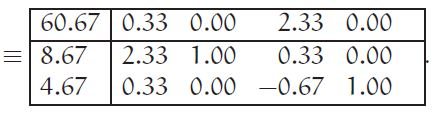
\includegraphics[width=0.7\linewidth]{Exam14-e}
\end{figure}
\end{frame}
%===============================================%
\begin{frame}
	\large
Explain why this Tableau is LP optimal. 1/2\%
\begin{itemize}
\item[(iii)] What is the solution to the LP Relaxation of the IP? 1/2\% \bigskip
\item[(iv)] Why must we now branch on x2 and what are the two branches? 1\%\bigskip
\item[(v)] Consider the right branch corresponding to a lower bound on x2
($x2 \geq ?$).
\end{itemize}

\end{frame}
%===========================================%
\begin{frame}
\large
\begin{itemize}
\item[A.] Amend the LP-optimal tableau T2 by adding an extra row \&
column corresponding to the extra constraint — creating a
new tableau T3 with 4 rows and 6 columns. (2\%) \bigskip
\item[B.] Perform one pivot on the appropriate element of T3 to eliminate
x2 from the new row. \\ \textit{N.B. Just update the last row,
not the full tableau. (1\%)}
\bigskip
\item[C.] Explain why the resulting tableau is infeasible. Update your
enumeration tree. (1\%)
\end{itemize}

\end{frame}
%===========================================%
%===========================================%
\begin{frame}
	
\begin{itemize}
\item[(vi)] Starting at T2, the left branch, $x_2 \leq 8$ (T4, say) (when the new
constraint is added and two pivots are performed) has the LP–
optimal tableau T4: (N.B. Do not perform the arithmetic!)
\end{itemize}


\end{frame}
%========================================== %
\begin{frame}
\begin{figure}
\centering
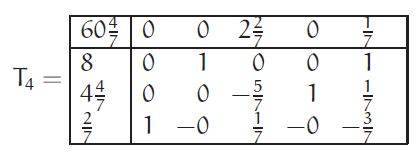
\includegraphics[width=0.7\linewidth]{Exam14-f}\\
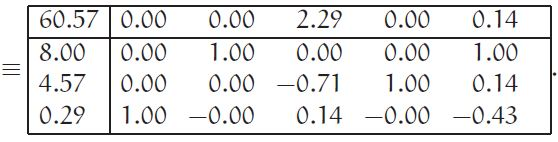
\includegraphics[width=0.7\linewidth]{Exam14-g}
\end{figure}
\end{frame}
%===========================================%
\begin{frame}
\large
Update your enumeration tree including the new upper bound on
the overall problem. Why must we now branch on x1 and what
are the two branches? 



% % 2015 
\end{frame}
%===========================================================================%
\begin{frame}
\begin{itemize}
\item[(vii)] Starting with T4, add a row corresponding to the left branch. Why
may we treat the new constraint as an equality constraint? 1%
\item[(viii)] Explain why we must pivot on the entry in row 4 and column 2 of
the resulting tableau. 1%
\item[(ix)] The tableau (T5 say) resulting from the extra row and the pivot is:
\end{itemize}

N.B. Do not perform the arithmetic!


\end{frame}
%================================================= %
\begin{frame}
Perform one step of the Dual Simplex Method and show that the
resulting tableau is \begin{figure}
\centering
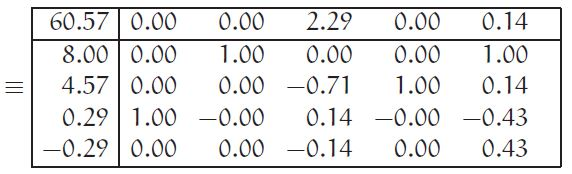
\includegraphics[width=0.7\linewidth]{Exam14-i}
\caption{}
\label{fig:Exam14-i}
\end{figure}

.
(Just calculate the first and fourth columns, columns 2 \& 3 do
not change. Columns 5 \& 6 are not needed.) 2%
\end{frame}
%================================================= %
\begin{frame}
(x) Finally; answer the following questions related to T6, briefly explaining your answer to each.
\begin{itemize}
\item[A.] What is the solution? 1/2\%
\item[B.] Is it IP optimal? 1/2\%
\item[C.] If possible update the global upper or lower bound on z? Explain
whicch can be updated. 1\%
\item[D.] Is the IP solved? If not, what other branch or branches must
be searched/fathomed/pruned? 1\%
\end{itemize}

\end{frame}

%========================================== %
%========================================== %
\end{document}
















(a) Apply one iteration of the Simplex Method to the starting tableau (T0)
and show that the Simplex Tableau now takes the form: 3\%
20 −3 0 2 0
10 −1 1 1 0
80 31 0 −16 1
\end{frame}
%==========================================================================%
\begin{frame}
(b) After a second iteration of the Simplex Method the Simplex Tableau
now takes the form: (N.B. Do not perform the arithmetic!)
T2 =
27.74 0 0 0.45 0.10
12.58 0 1 0.48 0.03
2.58 1 0 −0.52 0.03
\end{frame}
%==========================================================================%
\begin{frame}
(i) Explain why this Tableau is LP optimal. 1%
(ii) What is the solution to the LP Relaxation of the IP? 1%
(iii) Why is this not IP-optimal? 1%
(iv) What bound can you conclude for the optimal value of the objective
for the original IP? 1%
%==========================================================================%

(v) What are the two possible branches on x1 and what are the two
possible branches on x2? 1%
(c) Consider the right branch corresponding to a lower bound on x2 (x2 ≥
?).
%==========================================================================%
(i) The LP-optimal tableau T2 must be amended by adding an extra
row & column corresponding to the extra constraint. Explain
carefully why the new tableau T3 (with 4 rows and 6 columns)
takes the form: 2%
T3 =
27.74 0 0 0.45 0.10 0
12.58 0 1 0.48 0.03 0
2.58 1 0 −0.52 0.03 0
−13 0 −1 0 0 1
(ii) Which element of T3 should you pivot on next? Explain carefully. 1%
%==========================================================================%
(iii) The resulting tableau is
T4 =
27.74 0 0 0.45 0.10 0
12.58 0 1 0.48 0.03 0
2.58 1 0 −0.52 0.03 0
−0.42 0 0 0.48 0.03 1
(iv) Explain carefully why T4 is infeasible and update your enumeration
tree. 1%
(d) Consider the left branch corresponding to an upper bound on x2 (x2 ≤
?).

%===========================================%

(i) The LP-optimal tableau T2 must be amended by adding an extra
row & column corresponding to the extra constraint. Explain
carefully why the new tableau T5 (with 4 rows and 6 columns)
takes the form: 2%
T5 =
27.74 0 0 0.45 0.10 0
12.58 0 1 0.48 0.03 0
2.58 1 0 −0.52 0.03 0
12 0 1 0 0 1
%==========================================================================%
(ii) Which element of T5 should you pivot on next? Explain carefully. 1%
(iii) The resulting tableau is
T6 =
27.74 0 0 0.45 0.10 0
12.58 0 1 0.48 0.03 0
2.58 1 0 −0.52 0.03 0
−0.58 0 0 −0.48 −0.03 1
Using the Dual Simplex Method, which element should you pivot
on next so that the tableau is LP-optimal? Explain carefully. 2%
%==========================================================================%

(iv) The resulting tableau is:
T7 =
27.20 0 0 0 0.07 0.93
12 0 1 0 0 1
3.20 1 0 0 0.07 −1.07
1.20 0 0 1 0.07 −2.07

%===========================================%

(v) Is T7 LP-optimal? Explain carefully. 1%
(vi) Is T7 IP-optimal? Explain carefully. 1%
(e) Consider the left branch corresponding to an upper bound on x1 (x1 ≤
?).
%=============================================================================%

(i) As T7 is not IP-optimal it must be amended by adding an extra row
& column corresponding to the extra constraint. Explain carefully
why the new tableau T8 (with 5 rows and 7 columns) takes the
form: 2%
T8 =
27.20 0 0 0 0.07 0.93 0
12 0 1 0 0 1 0
3.20 1 0 0 0.07 −1.07 0
1.20 0 0 1 0.07 −2.07 0
3 1 0 0 0 0 1
%==========================================================================%
(ii) Which element of T8 should you pivot on next? Explain carefully. 1%
%==========================================================================%
(iii) The resulting tableau is
T9 =
27.20 0 0 0 0.07 0.93 0
12 0 1 0 0 1 0
3.20 1 0 0 0.07 −1.07 0
1.20 0 0 1 0.07 −2.07 0
−0.20 0 0 0 −0.07 1.07 1
%==========================================================================%
(iv) Using the Dual Simplex Method, which element of T9 should you
pivot on next? Explain carefully. 1%

(v) The resulting tableau is:
27 0 0 0 0 2 1
12 0 1 0 0 1 0
3 1 0 0 0 0 1
1 0 0 1 0 −1 1
3 0 0 0 1 −16 −15
%==========================================================================%
(vi) Does this tableau represent the optimal solution to the IP? Explain
carefully why or why not. 1%
(vii) What are the solution x and the objective value z associated with
the tableau? 1%
